\documentclass{standalone}
\usepackage{tikz-network}
\begin{document}
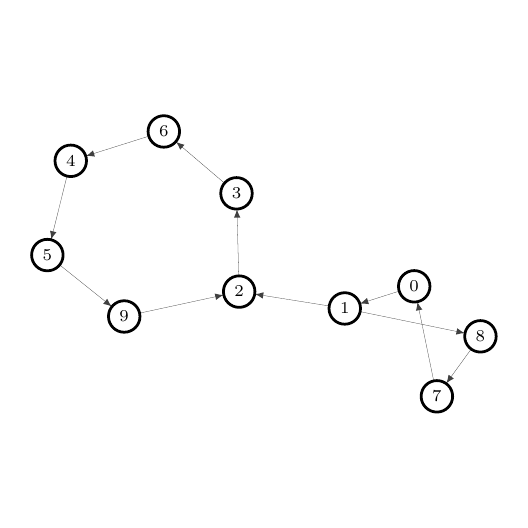
\begin{tikzpicture}
\clip (0,0) rectangle (6,6);
\Vertex[x=4.909,y=2.715,size=0.4,color=white,label=0,fontscale=0.857,shape=circle]{0}
\Vertex[x=4.027,y=2.434,size=0.4,color=white,label=1,fontscale=0.857,shape=circle]{5}
\Vertex[x=2.686,y=2.648,size=0.4,color=white,label=2,fontscale=0.857,shape=circle]{1}
\Vertex[x=2.652,y=3.896,size=0.4,color=white,label=3,fontscale=0.857,shape=circle]{3}
\Vertex[x=0.547,y=4.309,size=0.4,color=white,label=4,fontscale=0.857,shape=circle]{2}
\Vertex[x=0.250,y=3.112,size=0.4,color=white,label=5,fontscale=0.857,shape=circle]{6}
\Vertex[x=1.729,y=4.682,size=0.4,color=white,label=6,fontscale=0.857,shape=circle]{9}
\Vertex[x=5.197,y=1.318,size=0.4,color=white,label=7,fontscale=0.857,shape=circle]{4}
\Vertex[x=5.750,y=2.080,size=0.4,color=white,label=8,fontscale=0.857,shape=circle]{8}
\Vertex[x=1.226,y=2.332,size=0.4,color=white,label=9,fontscale=0.857,shape=circle]{7}
\Edge[,lw=0.1,bend=0,Direct](0)(5)
\Edge[,lw=0.1,bend=0,Direct](5)(1)
\Edge[,lw=0.1,bend=0,Direct](5)(8)
\Edge[,lw=0.1,bend=0,Direct](1)(3)
\Edge[,lw=0.1,bend=0,Direct](3)(9)
\Edge[,lw=0.1,bend=0,Direct](2)(6)
\Edge[,lw=0.1,bend=0,Direct](6)(7)
\Edge[,lw=0.1,bend=0,Direct](9)(2)
\Edge[,lw=0.1,bend=0,Direct](4)(0)
\Edge[,lw=0.1,bend=0,Direct](8)(4)
\Edge[,lw=0.1,bend=0,Direct](7)(1)
\end{tikzpicture}
\end{document}